
\chapter{The Standard Model of Particle Physics}
The aim of this chapter is to give a summary of the theoretical framework that is used in particle physics.
This framework was developed in stages throughout the latter half of the 20th century and is known as the Standard Model of particle physics.
The Standard Model is a quantum field theory which is able to describe most of what is seen in particle physics experiments and proved to be successful in predicting later experimental discoveries.
In this chapter a brief historical overview of the development of this theory will be given together with a limited description in order to familiarize the reader with concepts that will be used throughout this work.
For a more in-depth and exhaustive discussion I refer to Refs. \cite{Povh,Peskin:1995ev,Agashe:2014kda,Bettini:2008zz}. \textcolor{red}{Sections bla bla bla}

\section{What we call matter: fermions}
\label{sec:fermions}
Physics (from Ancient Greek: \gr φυσική \en - $physik\acute{\bar{e}}$, ``knowledge of nature'') is the natural science that studies matter.
Matter is made up by \textit{atoms} (from Greek: \textit{atomos}, ``indivisible'')\footnote{Coined by ancient Greek philosophers Leucippus and his pupil Democritus who believed matter was made up of discrete units.} which can bind together into molecules which results into what is around us in our everyday life.
Atoms are made up of a positively charged \textit{nucleus} and surrounded by one or more \textit{electrons} which are bound to the nucleus.
The nucleus is made up of one or more \textit{protons} and typically an approximately equal amount of \textit{neutrons}. Because of their similar characteristics protons and neutrons are often referred to as \textit{nucleons} and together they make up of more than 99.94\% of an atom's mass.
Nucleons are made up of smaller particles called \textit{quarks}\footnote{The word ``quark'' originally appeared in the novel \textit{Finnegans Wake} written by the Irish author James Joyce (1882–1941). The protagonist of the book dreams that he is serving beer to a drunken seagull. Instead of asking for ``three quarts for Mister Mark'' the inebriated bird says ``three quarks for Muster Mark''. Murray Gell-Man had the habbit of using names like ``squeak'' and ``squork'' for peculiar objects and after encountering the sentence in the book the name struck him ass appropriate since the hypothetical came in threes.} which are, as far as we know, \textit{fundamental particles}. This means that we believe there are no smaller substructures making up these objects and are in essence mathematically best described as infinitely small.
Because of this they are often referred to as pointlike.
In the Standard Model (SM) these particles are characterized in our three-dimensional space as \textit{fermions} which have odd half-integer spins obeying the laws of quantum mechanics.
The spin of a particle is often illustrated with it's classical counterpart in which an object is spinning and thus carries an intrinsic angular momentum.
This analogy cannot be extrapolated to pointlike particles but the property happens to hold the same units as the classical orbital momentum.
The spin of a particle seems to be just another property particles have, like charge or mass.
Fermions follow Fermi-Dirac statistics and therefore obey the Pauli exclusion principle. As a consequence fermions cannot occupy the same place at the same time. (More formally, no two fermions may be described by the same quantum numbers.) This agrees with our macroscopic obeservations of matter in everyday life: people cannot walk through walls!

In total the SM distinguished 24 different fermions which can be subdivided into two distinct classes: \textit{quarks} and \textit{leptons}. There are six quarks (up, down, charm, strange, top and bottom), and six leptons (electron, electron neutrino, muon, muon neutrino, tau and tau neutrino), along with the corresponding antiparticle of each of these.
A summary of the particles in the Standard Model is given in Figure \ref{SMparticles}.

\subsection{Leptons}
Leptons\footnote{\gr λεπτός \en (leptos) meaning thin, delicate, lightweight, or small. These particles don't need to bind to each other, which keeps them "thin" in a certain sense. Originally leptons were considered the "light" particles and hadrons the "heavy" particles, but the discovery of the tau lepton in 1975 broke that rule} can be subdivided into two classes: electromagnetically charged particles ($e$, $\mu$ and $\tau$) and the neutral neutrinos ($\nu_{e}$, $\nu_{\mu}$ and $\nu_{\tau}$). Because of their charge, electrons are the well known particles combining into atoms together with nucleons. Being the lightest of the three, the electron is said to be part of the first \textit{generation} together with the electron neutrino. Muons differ only from electrons in mass\footnote{This characteristic of often referred to as \textit{lepton universality} \cite{???}} and make up the second generation together with muon neutrinos. Similarly tau particles and tau neutrinos define the third generation. All leptons have a corresponding antiparticle indicated by a positive charge (i.e. $e^+$) or a bar (i.e. $\bar{\nu_e}$.). Neutrinos\footnote{The name is a worldplay. The Italian word for neutron (neutrone) sounds like the word neutral (neutro) with an augmentative suffix (-one) tacked on the end. That is, it sounds something like "big neutral" to Italian ears. Replace the augmentative suffix -one with the diminutive suffix -ino and you have a "little neutral", which is a good description of what a neutrino is — a diminutive neutral particle.} are proven to have a very small mass \textcolor{red}{REFERENCE} and interact only using the weak force (Section \textcolor{red}{HE?}) making them inherently very hard to detect.

\subsection{Quarks}
The six quarks are called up, down, charm, strange, top and bottom quarks $((u,d),(c,s),(t,b))$.
One generation is made up of a particle with charge 1/3 and one with 2/3. This is again visualized in Figure \ref{SMparticles}.
The difference between generations is essentially again the bare mass of the particles. Because quarks also interact through the strong force (see Section \textcolor{red}{????}) they combine into 
\textit{hadrons\footnote{\gr αδρός \en (adros) meaning thick, robust, massive, or large. This name alludes to the ability of the point-like quarks to bind together and form particles that are "thick" in a certain sense.}} of which the nucleons are best known. Because of their color charge and the intrinsic behaviour of the strong force quarks cannot be observed freely: they always combine into color neutral particles, a property called \textit{confinement}. Antiparticles are again denominated with a bar (i.e. $\bar{u}$). Because of their ability to interact with the strong force; particle accelerators in the 19???'s led to the discovery of a plethora of possible combinations. Something which is often referred to as the ``particle zoo''.

\begin{figure}
\label{SMparticles}
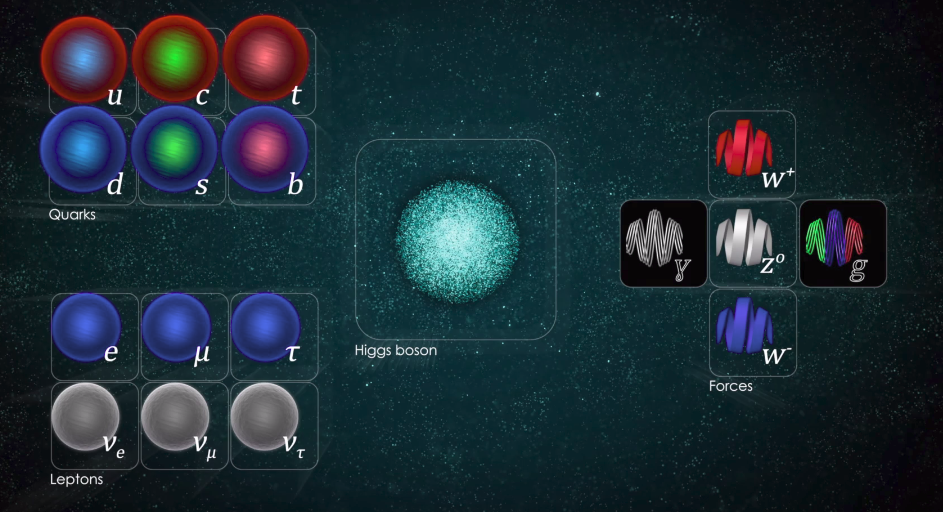
\includegraphics[width = \textwidth]{SMparticles}
\caption{info from: https://home.cern/about/physics/standard-model}
\end{figure}

\section{How particles communicate: interactions}

There are four fundamental interactions known to exist: gravity and electromagnetism, which produce significant long-range forces, and the strong and weak force which only express themselves at (sub)atomic distances and govern nuclear interactions. These are explained in more detail below and an overview is given in Table \ref{tab:forces}.

Particles interact with each other through the exchange of \textit{gauge bosons} or \textit{force carries}\footnote{A classic way of looking at force carriers is imagining two people standing in a boat. The force carrier is a heavy ball which can be thrown from one person to the other. Doing so both persons will move in opposite direction.}. Gauge bosons are bundles of energy (\textit{quanta}) and can be seen as excitations of one of the force fields.
Fields are a mathematical approach used by physicists to describe what we observe in exeriments.

Although the use of fields is very natural, the concept might feel a bit unfamiliar. In the following the known forces are described in more detail. Altough it plays less of a role in subatomic physics, the theory of gravity is added for completeness but is mainly used to explain the concept of fields more in depth.

\begin{table}[]
\label{tab:forces}
\begin{scriptsize}
\begin{tabular}{|l|c|c|c|c|c|}
\hline
\rowcolor{grey}
       &       & Weak                       & Electromagnetic      & \multicolumn{2}{|c|}{Strong}                            \\ \cline{3-6}
\rowcolor{grey}
\multirow{-2}{*}{\textbf{Interaction}}      & \multirow{-2}{*}{Gravitation} & \multicolumn{2}{|c|}{Electroweak}                                     & Fundamental    & Residual                   \\ \hline \hline
\cellcolor{grey} Acts on:                & Mass/Energy      & Flavor                     & Electric charge      & Color charge   & Atomic nuclei              \\ \hline
\cellcolor{grey}Particles experiencing: & All particles    & All fermions               & Electrically charged & Quarks, Gluons & Hadrons                    \\ \hline
\cellcolor{grey}Particles mediation:    & Not yet observed & $W^+,W^-, Z$               & $\gamma$ (photon)    & Gluons         & $\pi, \rho, \omega$ mesons \\ \hline
\cellcolor{grey}Strength                & $10^{-36}$       & $10^{???}$                 & 1                    & ???            & ???                        \\ \hline
\cellcolor{grey}Long-distance behaviour & $\frac{1}{r^2}$  & $\frac{1}{r}e^{-m_{W,Z}r}$ & $\frac{1}{r^2}$      & \multicolumn{2}{|c|}{$r$\footnote{One has to account for \textit{confinement}}}      \\ \hline
\end{tabular}
\end{scriptsize}
\caption{Bla bla bla. Ref: https://web.archive.org/web/20160304133522/https://www.pha.jhu.edu/~dfehling/particle.gif. A nice webpage explaining... :https://profmattstrassler.com/articles-and-posts/particle-physics-basics/the-known-forces-of-nature/the-strength-of-the-known-forces/
}
\end{table}


%Fields permiates through all of what we know ??? Similarly to particles fields are around us everywhere. For example: when you hold two magnets close together, you can feel their attraction or repulsion before they even touch - an interaction between two magnetic fields. Likewise, you know that when you jump in the air, you’re going to come back down. That’s because you live in Earth’s gravitational field.

\subsection*{Gravity}
Gravity (from Latin/old French: gravitas/grave, ``weighty, heavy'') is the phenomenon in which objects with mass are attracted to each other. Gravitation is famously described by the general theory\footnote{A scientific theory is an explanation of an aspect of the natural world that can be repeatedly tested, in accordance with the scientific method, using a predefined protocol of observation and experiment. Established scientific theories have withstood rigorous scrutiny and embody scientific knowledge. \textcolor{red}{REF WIKI?}} of general relativity proposed by Albert Einstein in 1915. Compared to the other forces gravity is intrinsically very weak\footnote{Two magnets that fit in the palm of your hand can deliver a force which is of similar strength than what the whole of Earth exerts on a human body.} and is not described in the SM (see Section???). Because of this, gravity is often left out in discussions of particle physics experiments. It can however be used to explain the concept of a field in a very natural way.

First published on July 5th 1686 in Newton's work \textit{Philosophiae Naturalis Principia Mathematica} (``the Principia''), a very good description of gravitation was already well known centuries ago. The equation of the force exerted by two massive bodies takes the following form:
\begin{equation}
F = G \frac{m_1 m_2}{r^2}
\end{equation}
where $F$ is the gravitational force acting between two objects, $m_1$ and $m_2$ are the masses of the objects, $r$ is the distance between the centers of their masses, and $G$ is the gravitational constant.

Newton's law states that two massive bodies will exert a force onto one another proportional to their masses but inversly proportional to the square of the distance between them. Newton realized this would mean that at any given instant in time this would mean that all massive objects in the universe would know of every other object in the universe where it is located\footnote{Imagine the attraction of the Moon towards the Earth: how are both ``communicating'' to each other?}. Because of this Newton himself believed his explanation could not be the final answer. The answer is fully described in Einstein's work\textcolor{red}{RELATIVITY} but was already explained by Pierre-Simon Laplace in 1783. Gravitation is the slope of a field that pervades space and because of this one only needs to know the value of the field in a local region to calculate the attractional force.
Massive objects do not ``feel'' each other but distort space and time in such a way that objects are attracted ``fall'' towards each other. Field theory makes it able to treat the laws of physics as local instead of action at a distance.


To date it is not possible for gravity to be described in the framework of quantum field theory like the other fundamental forces in a compatible way with the theory of general relativity. The gauge bosons from such a quantum field theory for gravity are referred to as \textit{gravitons}.

\subsection*{Electromagnetism}
The electromagnetic field (from Ancient Greek: \gr ἤλεκτρον \en $\bar{e}lektron$, "amber", and \gr μαγνῆτις λίθος, \en $magnetis lithos$, which means ``Magnesian stone'')\footnote{In 1641 Athanasius Kircher titled one of the chapters in his book Magnus \cite{BLABLABLA}: "Elektro-magnetismos i.e. On the Magnetism of amber, or electrical attractions and their causes" in which the ???} presents itself in the electrical and magnetical forces. In the late 1870's the publication of James Clerk Maxwell's \textit{A Treatise on Electricity and Magnetism} showed that the interactions of negative and positive charges are mediated by one force. Particles carrying a quantity (charge) of one of these forces can attract each other or repel.

Similar to the theory of gravity, the electromagnetic field pervades all around us and the interaction of nuclei, which have a positive electric charge, and electrons makes up most of what is described in chemistry. The force carrier of electromagnetism is called a \textit{photon}, or in other words: light.
\subsection*{Weak force}
The weak force is one aspect of the overarching electroweak theory which combines electromagnetism and the weak force. As opposed to gravity and electromagnetism it only takes place at very small subatomic distances\footnote{The reason being that the force carriers are massive, see more info in section???}. One well known phenomenon that is described by the weak force is \textit{beta decay} in which free neutrons decay into protons and produce an extra electron and anti-electron neutrino. Another beautiful example of the weak force is the driving mechanism in the Sun's thermonuclear process which makes it shine. This process cannot be explained by chemical processes but with the fusion of hydrogen into deuterium. Two protons are squeezed together into a He atom which consists of a proton and a neutron. The conversion of the proton into a neutron can be explained by the weak force.

The force carriers of the weak force are the $W^+$, $W^-$ and $Z$ bosons. Because of the mass of these particles the coupling of particles with the weak field is inversely proportional to the square of their mass the force seems to be very weak, hence it's name\footnote{Iets van Fermi?  Dat hij dacht dacht het een eenpuntsinteractie was?}.\\
The weak force also carries some peculiar properties which are unique in a number of respects:
\begin{itemize}
\item It is the only theory that violates parity symmetry and even does so maximally.
\item It's force carriers are massive as opposed to all other force carriers.
\item It is the only force capable of changing quarks from one family into a quark of another family.
\end{itemize}

\subsection*{Strong force}
As indicated in Section \ref{sec:fermions} nuclei are made up of protons and neutrons. However, the forces described in this section up to now cannot explain how they can make up a stable combination. The positive/neutral electromagnetic charge of the protons/neutrons would even suggest the opposite. Protons and neutrons are made up by quarks which carry a quantity which is called \textit{color charge}. Particles carrying a color charge participate in interactions of the strong force. Due to the principle of \textit{self interaction} the strong force only manifests itself on very small scales\footnote{As opposed to the weak force where the short distance is explained due to the mass of the force carriers.}. When nucleons are squeezed together (either due to high temperatures or pressure) and come close enough the quarks that make up the nucleons interact and make up the binding energy between nucleons.
The force carriers of the strong force are called \textit{gluons} which carry a color charge themselves and are massless.

Aside from holding nucleons together the strong force is also responsible for around 99\% of the mass of the nucleon mass. The binding energy (which includes the kinetic energy of the quarks and the energy of the gluon fields that bind the quarks together).

\section{The Standard Model in theory}
A lot from Mandel and Saw: QFT

The standard model is a \textit{quantum field theory}, meaning its fundamental objects are fields of a quantum nature which are defined at all points in spacetime. These fields are
\begin{itemize}
\item fermion fields, $\psi$, which account for ``matter particles'';
\item electroweak boson fields, $W^1, W^2, W^3$ and $B$;
\item gluon field, $G^a$; and
\item Higgs field, $\phi$
\end{itemize}
Quantum field theory treats particles as excited states of one of these underlying fields, so called \textit{field quanta}. The difference between classical and quantum fields is that they are operator-valued. Classical fields can in principle take on distinct values at each point in space whereas a quantum field accomodates oberservations of quantum mechanics as:
\begin{itemize}
\item energies are quantized, meaning that only discrete energy values are possible,
\item these discrete energy levels are equally spaced,
\item the lowest achievable energy is not equal to absolute zero, but has a zero-point energy\footnote{This is in accordance with the well known Heisenberg uncertainty principle which states that because of the zero-point energy, the position and momentum of a particle are not fixed but have a small range of variance: $\sigma_x\sigma_p \geq \frac{\hbar }{2}$.} (REFERENCE)?.
\end{itemize}

REFERENCE: https://arxiv.org/pdf/hep-ph/0609174.pdf,chapter 2
The dynamics of the quantum state and the fundamental fields are determined by the Lagrangian density $\mathcal{L}$. Writing the time and space coordinates in the form $(t,\mathbf{x}) = (x^0, x^1, x^2, x^3) = x^\mu$ the equations of motion of these fields can be written as:
\begin{equation}
\frac{\partial}{\partial x_{\mu}}\left[\frac{\partial \mathcal{L}}{\partial\left(\partial\phi/\partial x^{\mu}\right)}\right] - \frac{\partial \mathcal{L}}{\partial \phi} = 0,
\end{equation}
which follow from the principle of least action REFERENCE. The langrangian function depends on the fields and how these fields change in spacetime: $\mathcal{L(\phi,\nabla\phi)}$. Quantization of these fields can be obtained by interpreting the coordinates and momenta as Heisenberg operators, and subjecting these these to canonical commutation relations REFRENENCE MANDEL AND SHAW. 

Furthermore the standard model is a gauge theory in which the Lagrangian is invariant under certain Lie groups (referred to as the symmertry group or the gauge group of the theory) of local transformations. For quantized gauge groups the quanta of the gauge fields are referred to as \textit{gauge bosons}. A gauge theory is a mathematical model that has a gauge freedom of some of the mathematical degrees of freedom are reduntant. In other words: different mathematical expressions describe the exact same physical system and in that sense unphysical. An experiment could never uniquely determine their values, even in principle. If the phase of the wavefunction is changed by a different amount at each point in spacetime and the physics remains unchanged, the Lagrangian is said to follow a \textit{local phase symmetry}.\footnote{See appendix A}.

The standard model is defined by the local SU(3) $\times$ SU(2) $\times$ U(1) gauge symmetry. Each factor gives rise to three fundamental forces:
\paragraph{SU(3): quantum chromodynamics}
The quantum chromodynamics (QCD) sector defines the interactions between quqrks and glons. Since leptons do not carry colour charge they do not participate in this interaction. The Dirac Lagrangian of the quarks coupled to the gluon fields is given by

\begin{equation}
\mathcal{L}_{QCD} = \sum_{\psi} \bar{\psi_i} \left(i \gamma^\mu \left(\partial_\mu  \delta_{ij} - i g_s G^a_{\mu} T^a_{ij}\right) - m_\psi \delta_{ij} \right) \psi_j - \frac{1}{4} G^a_{\mu\nu}G^{\mu\nu}_a,
\end{equation}
where\\
\indent $\psi_i$ is the Dirac spinor of the quark field, where $i=${r,g,b} represents the color charges,\\
\indent $\gamma^\mu$ are the Dirac matrices REFERENCE,\\
\indent $G^a_\mu$ is the 8-component $\left(a=1,2,...,8\right)$ SU(3) gauge field,\\
\indent $T^a_{ij}$ are the $3\times3$ Gell-Mann matricesREF, generators of the SU(3) color group,\\
\indent $G^a_{\mu\nu}$ are the field strength tensors for the gluons,\\
\indent $g_s$ is the strong coupling constant.

\paragraph{SU(2) $\times$ U(1): electroweak}
The electroweak sector is a Yang-Mills gauge theoryREF with the symmetry group SU(2)$_L$ $\times$ U(1). The Lagrangian is given by

\begin{equation}
\begin{split}
\mathcal{L}_{EW} &= \sum_{\psi} \bar{\psi} \gamma^\mu \left(i\partial_\mu - g' \frac{1}{2}Y_W B_\mu - g \frac{1}{2} \overrightarrow{\tau_L} \overrightarrow{W}_\mu \right) \psi - \frac{1}{4} W^{\mu\nu}_a W^{a}_{\mu\nu} -\frac{1}{4} B^{\mu\nu} B_{\mu\nu} \\ 
&= \bar{Q}_i i D_\mu \gamma^\mu Q_i + \bar{u}_i i D_\mu \gamma^\mu u_i + \bar{d}_i i D_\mu \gamma^\mu d_i + \bar{L}_i\left(iD_\mu\gamma^\mu\right)L_i + \bar{e}_{R,i}\left(iD_\mu\gamma^\mu\right)e_{R,i} \\ &
- \frac{1}{4} W^{\mu\nu}_a W^{a}_{\mu\nu} -\frac{1}{4} B^{\mu\nu} B_{\mu\nu},
\end{split}
\end{equation}
where\\
\indent $B_\mu$ is the U(1) gauge field,\\
\indent $Y_W$ is the weak hypercharge - the generator of the U(1) group,\\
\indent $\overrightarrow{W}_\mu$ is the 3-component SU(2) gauge field,\\
\indent $\overrightarrow{\tau_L}$ are the Pauli matrices - infinitesimal generators of the SU(2) group - with subscript L to indicate that they only act on left-chiral fermions,\\
\indent $g'$ and $g$ are the U(1) and SU(2) coupling constants respectively,\\
\indent $W^{a\mu\nu} (a=1,2,3)$ and $B^{\mu\nu}$ are the field strength tensors for the weak isospin and weak hypercharge fields\\
\indent $Q, u$ and $d$ are the left-handed doublet, right-handed singlet up right-handed singlet down quark fields,\\
\indent $L$ and $e$ are the left-handed doublet and right-handed singlet electron fields.

It is worth noting no terms are included for fermion masses. These would have the form of $m\bar{\psi}\psi$ but are forbidden as they would break the SU(2)$_L$ $\times$ U(1) gauge invariance. Neither is it possible to add explicit mass terms for the U(1) and SU(2) gauge fields. 
\paragraph{Brout-Englert-Higgs mechanism}
To come to a viable description of the elementary particles one is required to introduce masses into a chiral theory.

To explain the masses of the $W$ and $Z$ bosons the Brout-Englert-Higgs mechanism formulation is used. By introducing one or more scalar fields, the Higgs fields, which can acquire a vacuum expectation value it is possible to spointaneously break a symmetry in the Lagrangian. According to the Goldstone theorem REF, every spontaneously broken continuous symmetry results in a massless scalar particle, the Goldstone boson. Hence, the number of Goldstone bosons in a theory is equal to the number of broken generators of the symmetry group.

Since the electroweak theory after symmetry breaking should contain three massive gauge bosons ($W^+, W^-$ and $Z$) the scalar fields of the Higgs fields should contain at least three degrees of freedom. The simplest approach to do this is by introducing a complex, scalar SU(2) doublet $\Phi$ with positive hypercharge $\left(Y=\frac{1}{2}\right)$,
\begin{equation}
\Phi = \begin{pmatrix} \phi^+ \\ \phi^0 \end{pmatrix}.
\end{equation}

Beautiful interplay of forces: i.e. strong force necessary to KEEP the neutrons as they are. Without it all neutrons would become protons! On the other hand; protons and neutrons would weigh the same if ....?

\section{How particles get their mass: the Brout-Englert-Higgs model}
Misschien toch eerst de harde wiskunde en dan pas BEH?

EM: all of chemistry

Strong interaction: like velcro: very very hard and then nothing

Weak interaction: a force that without it, the sun would not shine

Strength of forces compared: gravity so weak also reason why we cannot study it and prob. why we don't really know what it is at quantum level

Force carriers: like throwing a ball when you're in a boat: changes your velocity, direction, energy,...

Fun fact: entire lagrangian somewhere in a footnote?

Gargamelle experiment: weak neutral currents: hint of Z boson discovery? Another decade for direct detection

Weak bosons: proof that there are 3 and only 3 families

Bosons, in contrast, are have no problem occupying the same place at the same time. (More formally, two or more bosons may be described by the same quantum numbers.) The statistical rules that bosons obey were first described by Satyendra Bose (1894–1974) of India and Albert Einstein (1879–1955) of Germany. Gluons, photons, and the W, Z and Higgs are all bosons. As the particles that make up light and other forms of electromagnetic radiation, photons are the bosons we have the most direct experience with. In our everyday experience, we never see beams of light crash into one another. Photons are like phantoms. One may pass through the other with no effect.



For those who like fancy math, the standard model is described using group theory notation as…

SU(3) x SU(2) x U(1)

where the gauge group of the strong interaction is…

SU(3)

and the gauge group of the electroweak interaction is…

SU(2) x U(1)

Notes…

SU(3)

\begin{comment}
3rd order special unitary group
the set of all 3 x 3 unitary matrices with unit determinant
SU(2)
2nd order special unitary group
the set of all 2 x 2 unitary matrices with unit determinant
isomorphic to the group of quaternions of absolute value 1, {x ∈ ℍ: |x| =1}
diffeomorphic to a hypersphere (3-sphere)
homomorphic to the rotation group SO(3), the set of all rotations about the origin in ordinary three dimensional euclidean space
U(1)
1st order unitary group
the set of all 1 × 1 unitary matrices
isomorphic to the circle group, the multiplicative group of complex numbers with absolute value 1, T = {x ∈ ℂ: |x| =1}
isomorphic to SO(2), the second order special orthogonal group
What is this? The Standard Model Lagrangian.

ℒ = −¼FμνFμν + iψ̄D̸ψ + ψiyijψjφ + h.c. + |Dμφ|2 − V(φ)
\end{comment}

Leuk: bestaat ook niet zoiets als negatieve zwaartekracht. Nochtans wel alle andere flavors negatief en positief

\chapterimage{Unifying_theories_gravity_is_difficult.pdf} % Chapter heading image